\documentclass[a4paper,francais]{insalyon}
\usepackage[utf8]{inputenc}
\usepackage[T1]{fontenc}
\usepackage[french]{babel}

\usepackage{subfig}
\usepackage{graphicx}
\graphicspath{{fig/}}

\usepackage{amssymb}
\usepackage{amsthm}

\usepackage{hyperref}

\usepackage{cprotect} %verbatim in footnote

\newcommand{\cad}{c.-à-d.}

\title{ELP}
\author{Tristan Roussillon}

\begin{document}

\maketitle

L'objectif de ce document est de présenter d'une façon simple dix thèmes centraux autour desquels se déroule l'activité de programmation. L'étudiant les découvre en général à l'occasion d'un projet ou d'un exercice et par le prisme d'un langage particulier. Il s'agit ici de les mettre en mots afin de l'aider à nommer et prendre conscience de ces éléments importants. 

\section{Les fondamentaux de l'informatique et la programmation}

L'informatique est une science dont l'objet d'étude est constitué de grands piliers : représentation de l'information, algorithme, language et machine \cite{rapportacscience} : 
%% \footnote{cf. le rapport de l'académie des sciences:
%%   \href{https://www.academie-sciences.fr/pdf/rapport/rads\_0513.pdf}
%%   {l'enseignement de l'informatique en France, il est urgent de ne plus attendre, mai 2013}.
%%   }.
\begin{description}
\item[information] (Larousse) Élément de connaissance susceptible d'être représenté à l'aide de conventions pour être conservé, traité ou communiqué. 
\item[algorithme] (\cite[p.4]{knuth}) Ensemble fini de règles qui fourni une séquence d'opérations. Ces opérations permettent d'obtenir, à partir de zéro ou plusieurs informations en entrée, au moins une information en sortie, qui est la réponse à un problème spécifique. Un algorithme doit de plus être précisément défini, sans ambiguité sur les actions à mener, et effectivement réalisable, dans le sens où l'exécution doit terminer après un nombre fini d'étapes, chaque étape étant suffisamment élémentaire pour pouvoir, en principe, être effectuée exactement, en un temps fini, par un opérateur humain.
  %Synonyme de recette, méthode, technique, procédure, 
\item[langage] Dans ce contexte, on appelle \emph{langage} un système de signe capable d'exprimer un algorithme. Il est doté d'une \emph{syntaxe} (en fonction des règles de sa \emph{grammaire}, certains agencements de signe sont admissibles et d'autres non) et d'une \emph{sémantique} (tous les agencements de signe admissibles ont une signification précise). Tous les langages n'ont pas le même pouvoir expressif ; seuls ceux dits complets au sens de Turing sont capables d'exprimer n'importe quel algorithme.  
\item[machine] Dans ce contexte, on appelle \emph{machine} tout dispositif capable de traduire un algorithme, exprimé dans un langage spécifique, en actions. L'orgue de barbarie, le métier à tisser Jacquart, l'ordinateur, le smartphone sont des exemples de machine. 
\end{description}

La programmation consiste à écrire des programmes, {\cad} exprimer des algorithmes dans un langage spécifique, afin d'adapter les actions exécutées par une machine. Elle est au c\oe ur de l'informatique. Du fait de l'omniprésence de l'informatique dans de nombreux domaines de l'activité humaine, elle est pratiquée par de nombreux ingénieurs. 

%https://fr.wikipedia.org/wiki/Langage
%https://fr.wikipedia.org/wiki/Langage_informatique
%https://fr.wikipedia.org/wiki/Langage_de_programmation
%https://fr.wikipedia.org/wiki/Langage_formel

\section{Compilation, exécution}

En informatique, dans son acception large, la compilation consiste en la traduction d'un programme écrit dans un langage, en un programme écrit dans un autre langage. Par exemple, j'ai rédigé ce que vous lisez en {\LaTeX} et j'ai utilisé l'outil \texttt{pdflatex} pour produire ce fichier \texttt{pdf} : \texttt{pdflatex document.tex} $\leadsto$ \texttt{document.pdf}
\footnote{Tous les exemples donnés dans ce document supposent un environnement Linux.}.  

Au sens strict, le produit de la compilation est un fichier binaire directement exécutable par l'ordinateur, voire un programme écrit dans un langage intermédiaire pouvant être exécuté par une machine virtuelle, {\cad} un logiciel émulant les fonctionnalités d'un ordinateur. Le \emph{compilateur} est le logiciel qui effectue une telle traduction. Ce traitement est habituellement terminé avant toute exécution du programme obtenu.

Dans d'autres cas, le programme source est analysé, traduit et exécuté petit à petit par un logiciel appelé \emph{interpréteur}.

Pour synthétiser, on peut retenir ceci :
\begin{description}
\item[compilé] ~\\ compilateur(programme source) $\leadsto$ fichier exécutable ; \\
  système d'exploitation(fichier exécutable) $\leadsto$ actions
\item[semi-compilé] ~\\ compilateur(programme source) $\leadsto$ programme intermédiaire ; \\
  machine virtuelle(programme intermédiaire) $\leadsto$ actions
\item[interprété] ~\\ interpréteur(programme source) $\leadsto$ actions
\end{description}

Même si un langage peut en théorie être aussi bien compilé ou interprété, il apparaît dans les faits avec une certaine implémentation. Voici quelques exemples.

\subsection{Exemples de programmes compilés}

Les programmes écrits en Haskell, Go, C peuvent être compilés respectivement avec les compilateurs ghc, golang-go, gcc.
Dans les exemples suivants, la commande de compilation, à laquelle on indique éventuellement le nom du programme source, est à gauche,
le nom du fichier exécutable produit est à droite :
\begin{itemize}
  \item \verb! ghc main.ghc ! $\leadsto$ \texttt{main}
  \item \verb! go build ! $\leadsto$ \texttt{hello}
    \footnote{ Le programme source, appelé obligatoirement \texttt{main.go}, se trouve dans un dossier appelé \texttt{hello} (nom donné au projet dans cet exemple ; le fichier exécutable prend le nom du projet), lui-même contenu dans un dossier \texttt{src} (car l'environnement Go suppose que tous les projets se trouvent dans un dossier appelé \texttt{src}. La commande de compilation \texttt{go build} est exécutée à la racine du projet, {\cad} dans le dossier \texttt{hello/src}. On voit ici qu'il y a toujours de nombreuses \emph{conventions} à connaître. }
  \item \verb! gcc main.c ! $\leadsto$ \texttt{a.out}
\end{itemize}

Les fichiers produits sont directement exécutables depuis le shell : 
\begin{itemize}
\item \verb! ./main ! $\leadsto$ actions
\item \verb! ./hello ! $\leadsto$ actions
\item \verb! ./a.out ! $\leadsto$ actions
\end{itemize}

Ces fichiers contiennent du \emph{code natif}, {\cad} un programme écrit dans un langage machine spécifique à l'environnement utilisé, à la fois en terme de système d'exploitation et d'architecture d'ordinateur. Un code natif est exécuté très rapidemment, mais ne pourra pas être exécuté sur une machine aux caractéristiques différentes de celle sur laquelle le code natif a été produit. 

\subsection{Exemple de programme semi-compilé}

Les programmes écrits en Java sont généralement compilés dans un premier en temps en \emph{byte code} par la commande \texttt{javac} :

\verb! javac Classe.java ! $\leadsto$ \texttt{Classe.class}

Dans un second temps, le \emph{byte code} est éxécuté par la machine virtuelle java, dont l'exécution est lancée par la commande \texttt{java} :

\verb! java Classe ! $\leadsto$ actions \footnote{On fournit à la commande \texttt{java} le nom complet de la classe et la machine virtuelle java charge en mémoire le byte code correspondant, contenu dans le fichier d'extension \texttt{.class}. }

C'est un compromis entre
\emph{portabilité} (le byte code produit peut être exécuté dans n'importe quel environnement pourvu qu'il y ait une machine virtuelle java\footnote{C'est ce qu'exprime le slogan ``Write once, run everywhere''.})
et \emph{rapidité d'exécution} (le byte code est suffisamment proche d'un code natif pour être exécuté relativement rapidement, d'autant que les machines virtuelles sont maintenant dotées de mécanisme de compilation à la volée pour traduire les parties du byte code les plus sollicitées en code natif).   

\subsection{Exemple de programme interprété}

\texttt{Node.js} est un interpréteur de programmes écrits en JavaScript :

\verb! node toto.js ! $\leadsto$ exécute ce qui est écrit dans le fichier \texttt{toto.js}

Les programmes interprétés sont généralement appelés \emph{scripts}. Leur exécution est plus lente, puisque l'analyse du script est effectuée au cours de l'exécution. En revanche, il est généralement possible d'exécuter des scripts incomplets, ce qui facilite leur incorporation dans d'autres contextes (HTML + JavaScript interprétés par un navigateur web par exemple). Cette souplesse accélère aussi le développement de prototypes d'application.


\section{Données}

%donnée une donnée est la représentation d'une information dans un programme : soit dans le texte du programme (code source), soit en mémoire durant l'exécution.
%https://fr.wikipedia.org/wiki/Donn%C3%A9e_(informatique)
Une \emph{valeur} est une donnée, {\cad} la représentation d'une information, aussi bien dans le texte du programme source, qu'en mémoire durant l'exécution. 
Un \emph{littéral} est une valeur écrite explicitement dans le programme source, comme 2, 5.7, True, "hello" ou encore
\begin{verbatim}
{ "nom" : "roussillon", "age" : 35 }.
\end{verbatim}
\'Evidemment, un programme ne contenant que des valeurs littérales ne serait pas très intéressant, car il ne serait pas capable d'adapter les actions de la machine en fonction d'informations données. Ce qui rend intéressant les programmes sont leurs variables. 
Une \emph{variable} représente une donnée susceptible de changer au cours de l'exécution ou d'une exécution à l'autre. Elle possède un nom, appelé aussi \emph{identifiant}, une \emph{valeur} stockée en mémoire au cours de l'exécution (et qui peut changer ou non), ainsi qu'un \emph{type} caractérisant les valeurs admissibles et les opérations pouvant leur être appliquées. Les variables ont également une durée de vie, appelée aussi \emph{portée}, en général limitée (pour ne pas conserver en mémoire une valeur qui serait devenue inutile).  
%compliqué à précisé. 
%qui peut être restreinte qui est le bloc, {\cad} la portion de programme bien délimitée, dans laquelle elle est déclarée ou utilisée pour la première fois.

Comme sur la \textsc{Figure}~\ref{fig:var}, la métaphore de la boite est largement utilisée en programmation. Une variable est considérée comme une boite bien identifiée, dans laquelle se trouve une (et une seule) valeur. Grâce au typage, la boite est dimensionnée aux valeurs susceptibles d'y être contenue. La plupart du temps, il est possible de remplacer la valeur qui se trouve dans une boite, par une autre : c'est \emph{l'affectation}. Il est aussi possible de ne pas fournir de valeur initiale à la création de la boite ; dans ce cas, elle n'est pas vide, mais contient une valeur arbitraire. Dans certains cas, parce qu'on le spécifie explicitement ou que c'est l'un des principes du langage, comme en Haskell, il est interdit de changer la valeur d'une variable.

\begin{figure}[htbp]
  \centering
  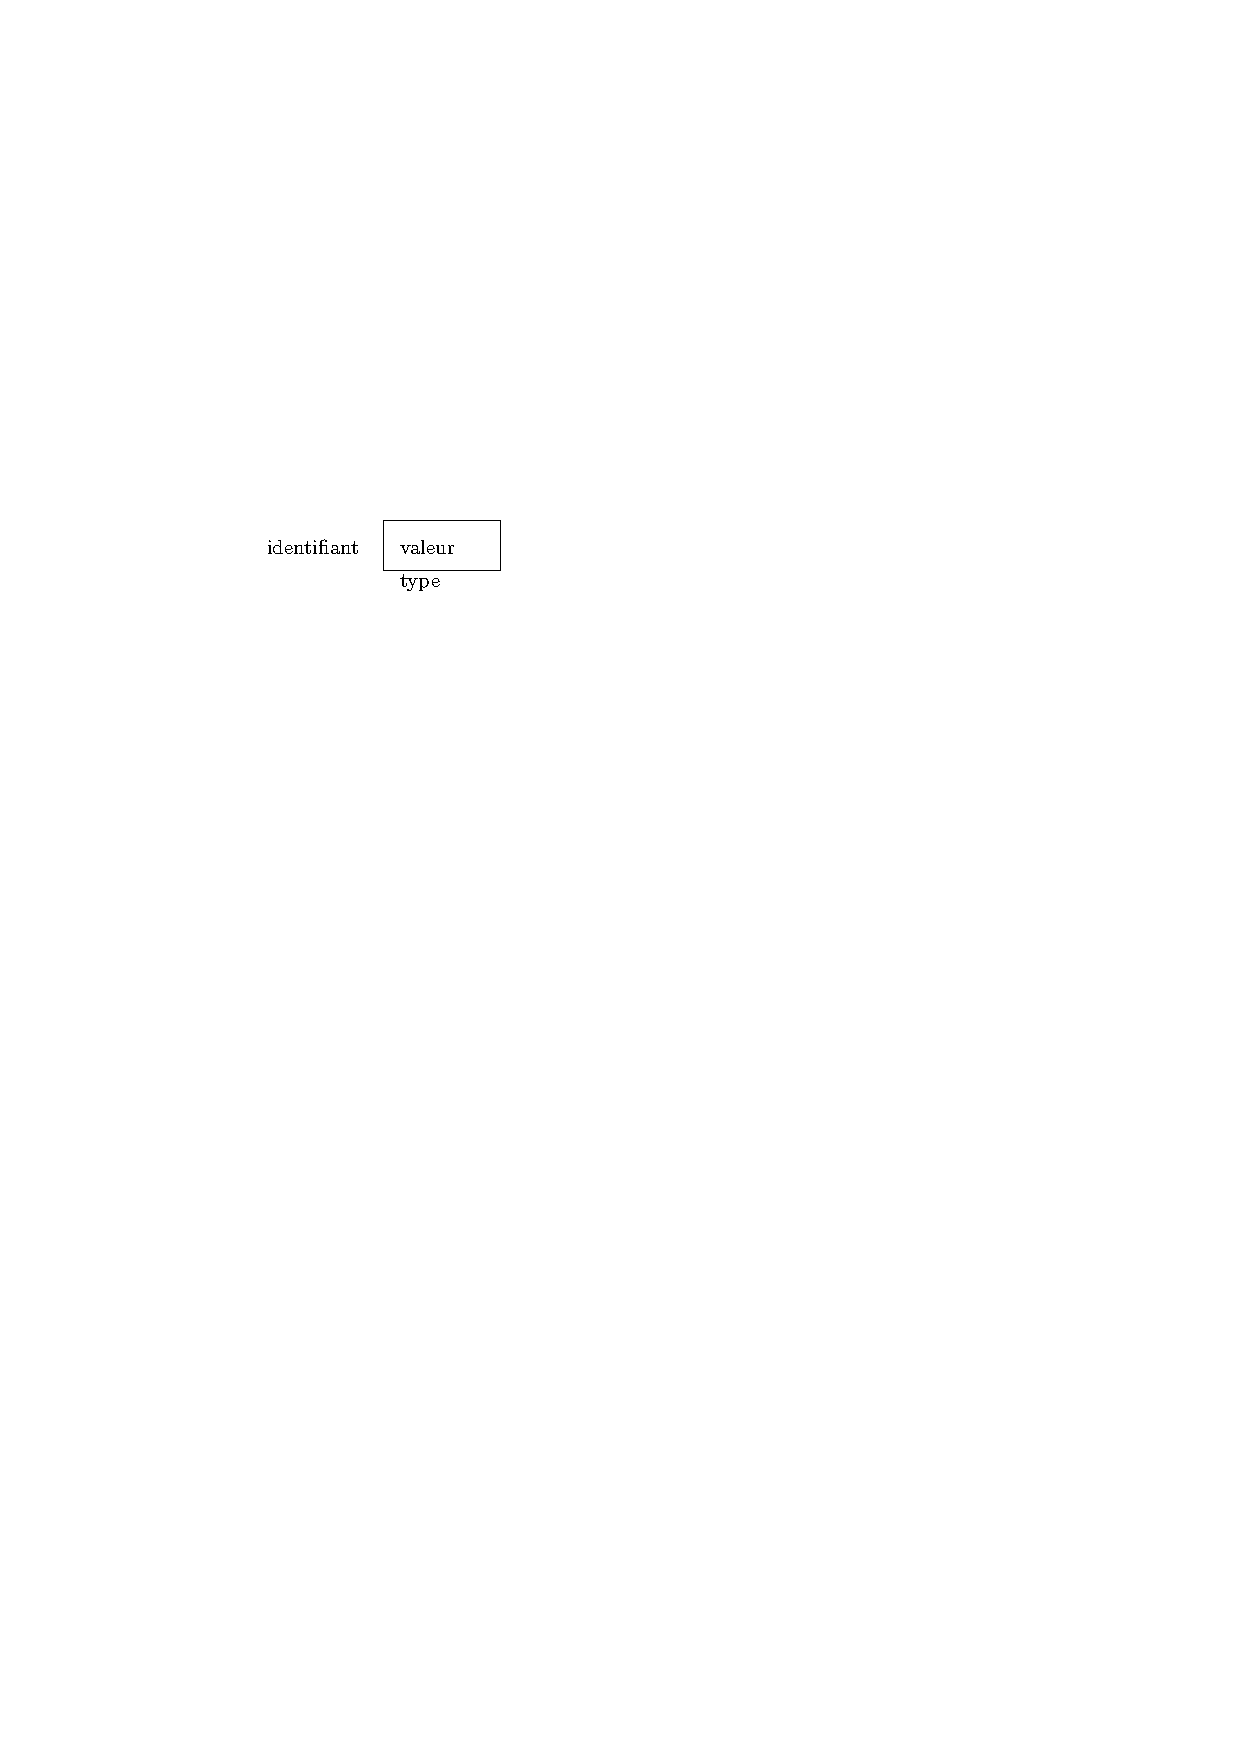
\includegraphics[width=5cm,page=1]{variable} \hspace{1cm}
  \includegraphics[width=5cm,page=2]{variable}
  \caption{Représentation schématique d'une variable.}
  \label{fig:var}
\end{figure}

\subsection{Types de base}

La plupart des langages offrent plusieurs types prédéfinis pour des valeurs élémentaires :
\begin{itemize}
\item le type booléen pour les valeurs de vérité vrai et faux, sur lesquelles agissent au moins les opérateurs booléens (\verb!negation, et, ou,! \ldots),
\item le type entier pour les nombres entiers, signé ou non, pouvant être codés sur 8, 16, 32 ou 64 bits et sur lesquels agissent au moins les opérateurs arithmétiques (\verb!+, -, *, modulo,! \ldots), 
\item le type réel pour des nombres décimaux, codés sur 32 ou 64 bits selon la représentation en virgule flottante de la \href{https://fr.wikipedia.org/wiki/IEEE_754}{norme IEEE 754}\footnote{A ce propos, \cite{goldberg91} est une lecture encore intéressante.} et sur lesquels agissent aussi des opérateurs arithmétiques (\verb!+, -, *, /,! \ldots),
\item le type caractère selon le standard \href{https://fr.wikipedia.org/wiki/American_Standard_Code_for_Information_Interchange}{ASCII} ou \href{https://fr.wikipedia.org/wiki/Unicode}{Unicode}, sur lequel agissent par exemple des opérateurs de comparaison (\verb!egalite, <, >,! \ldots).
\end{itemize}

Il est aussi souvent possible de définir de nouveaux \emph{types énumérés} pour lesquels on donne explicitement toutes les valeurs possibles. Ces valeurs sont en général automatiquement mises en correspondance avec des entiers naturels, mais les nommer permet d'ajouter de la sémantique. Le type \texttt{JourDeLaSemaine}, par exemple, pourrait être défini comme n'acceptant que les valeurs \verb!Lundi, Mardi,! \ldots \verb!, Dimanche!. Les valeurs \verb!1, 2,! \ldots \verb!, 7! d'un type entier, même accompagnées de documentation, ne porteraient pas une signification aussi transparente.    

\subsection{Types composés}
\label{sec:types-composes}

La plupart des langages de programmation proposent également des types composés, pouvant être paramétrés ou personnalisés, pour des valeurs structurées :
\begin{itemize}
\item Les types \emph{tableau} et \emph{liste}, sont paramétrés par un type \texttt{t} et acceptent une séquence de valeurs du même type \texttt{t} (\texttt{t} est arbitraire, avec parfois des restrictions). L'opérateur d'accès à une valeur de la séquence est souvent noté par des crochets : \verb! unTableau[3] ! retourne la valeur de rang 3 dans la séquence. Les valeurs sont stockées en mémoire les unes à côtés des autres dans le cas des tableaux, tandis qu'elles peuvent être dispersées dans le cas des listes (\textsc{Figure}~\ref{fig:types}(a) et (b)). Cela à un impact sur la rapidité des traitements : l'accès est garanti en un nombre constant d'opérations élémentaires dans le cas des tableaux, alors qu'il peut nécessiter la visite de toutes les valeurs, l'une après l'autre, dans le cas d'une liste, ce qui implique un nombre d'opérations élémentaires proportionnel à la taille de la liste.
\item Il existe aussi des types composés non homogènes qui acceptent une collection de valeurs, appelées \emph{champs}, de types possiblement différents les uns des autres (voir la \textsc{Figure}~\ref{fig:types}(c), ainsi que l'annexe~\ref{a:enregistrement}). Ils sont généralement appelés \emph{tuple} quand les champs ne sont pas nommés (Haskell, Python), \emph{struct} ou \emph{enregistrement} quand ils le sont (C, Go, Haskell). L'appelation \emph{type produit} aussi utilisée en Haskell vient de ce que l'ensemble des valeurs admises par un tel type sont composées des valeurs des types de ses champs selon le produit cartésien. Par exemple, le type \verb!(booléen, booléen)! représente toutes les combinaisons de deux valeurs de type booléen, soit l'ensemble $\{ (vrai, vrai), (vrai, faux), (faux, vrai), (faux, faux) \}$\footnote{J'ai volontairement choisi deux champs de type booléen pour aisément énumérer l'ensemble des valeurs possibles du type produit, mais le principe est le même pour un nombre arbitraire de champs de type différent. Il est par exemple tout à fait possible d'avoir un premier champs de type entier, un deuxième de type caractère, voire un troisième de type liste, \ldots}   
\item Les \emph{types algébriques}, en référence aux structures algébriques mathématiques, sont des unions disjointes de types produits. Une présentation détaillée des types algébriques en Haskell se trouve par exemple dans \cite[chapitre 3]{haskell}.    
\item Les \emph{classes} (en Java par exemple, mais plus généralement en programmation orientée objet) représentent aussi une collection de \emph{champs} (comme des enregistrements), mais possiblement enrichies des fonctions, appelés dans ce contexte \emph{méthodes}, qui agissent sur cette collection. Les concepts de fonction et méthode sont comparés dans la section~\ref{sec:fonction-methode}.
\end{itemize}

\captionsetup[subfigure]{labelformat=empty}
\begin{figure}[htbp]
  \centering
  \parbox[b]{7cm}{
    \subfloat[(a)]{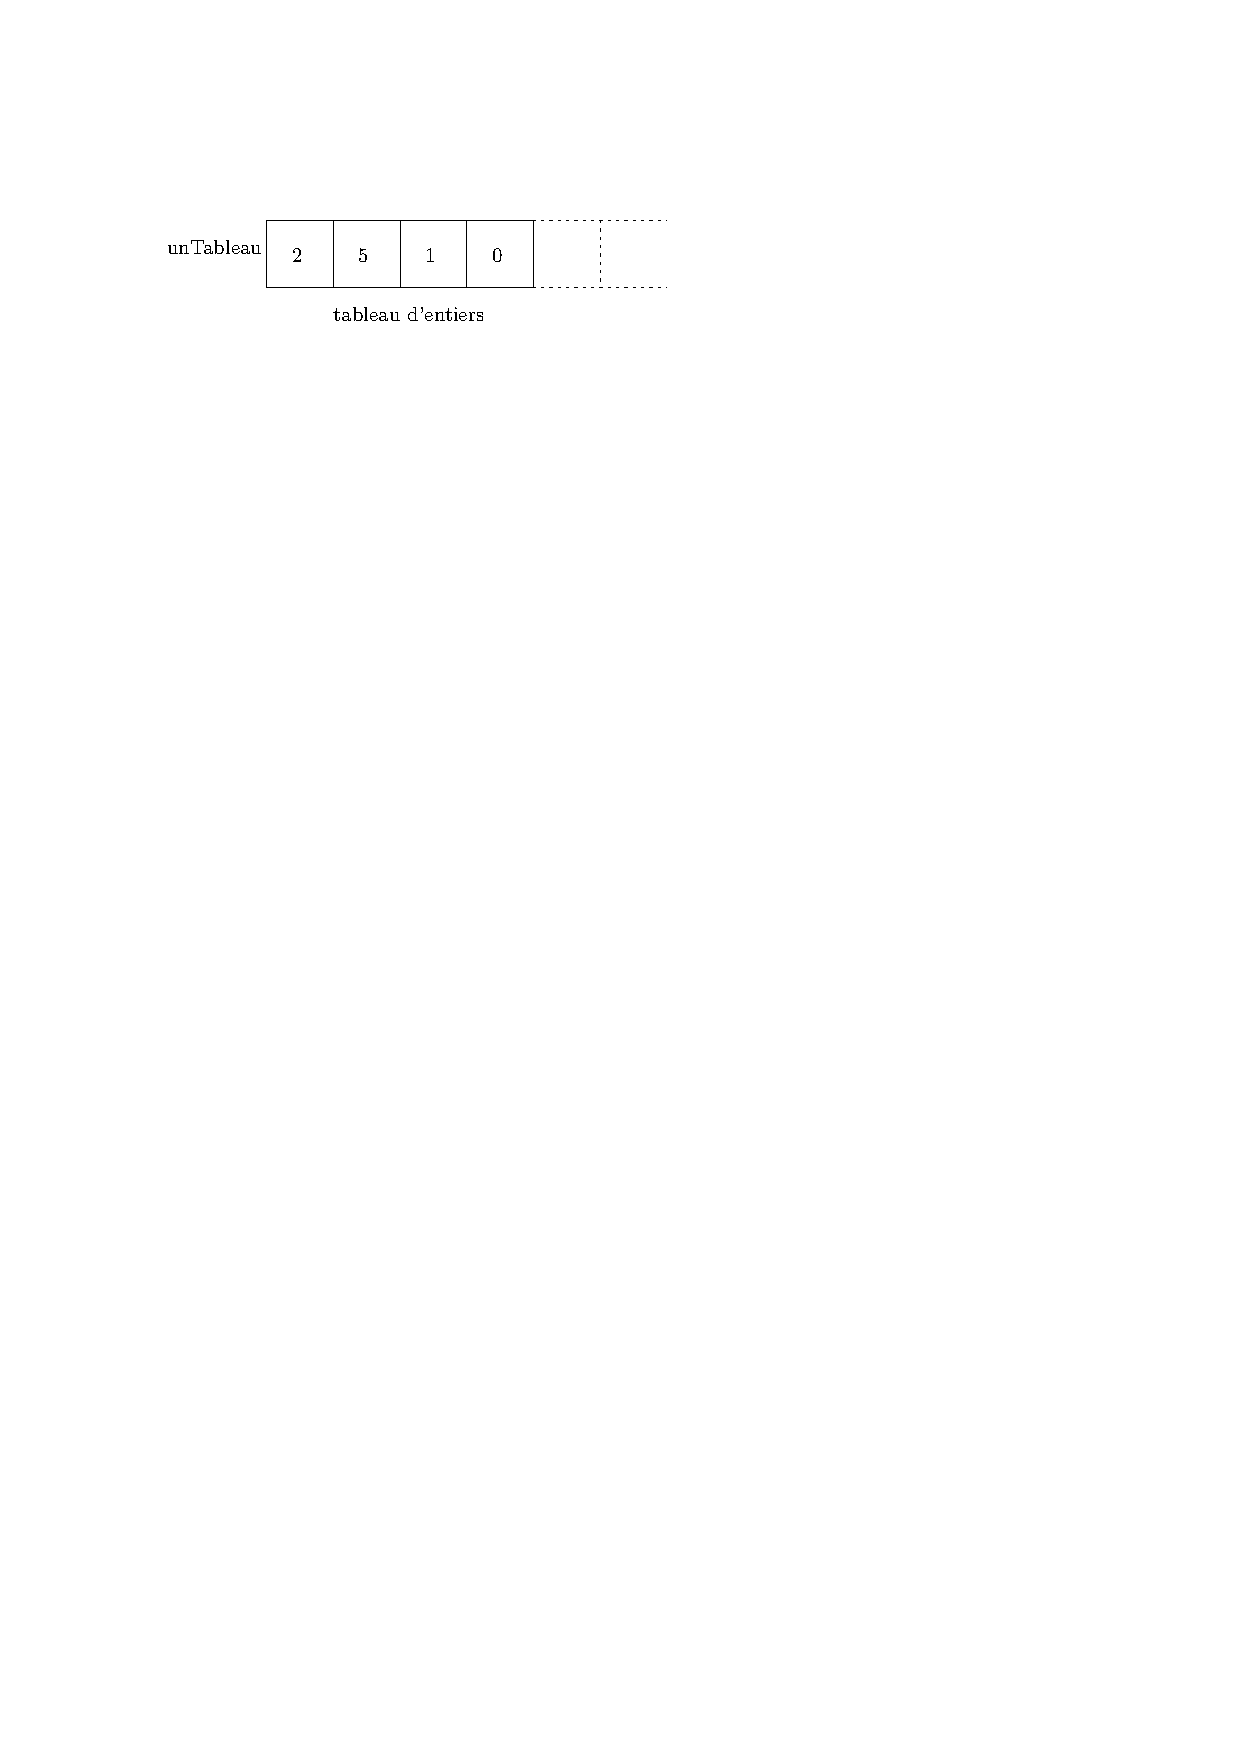
\includegraphics[width=7cm]{tableau}} \\
    \subfloat[(c)]{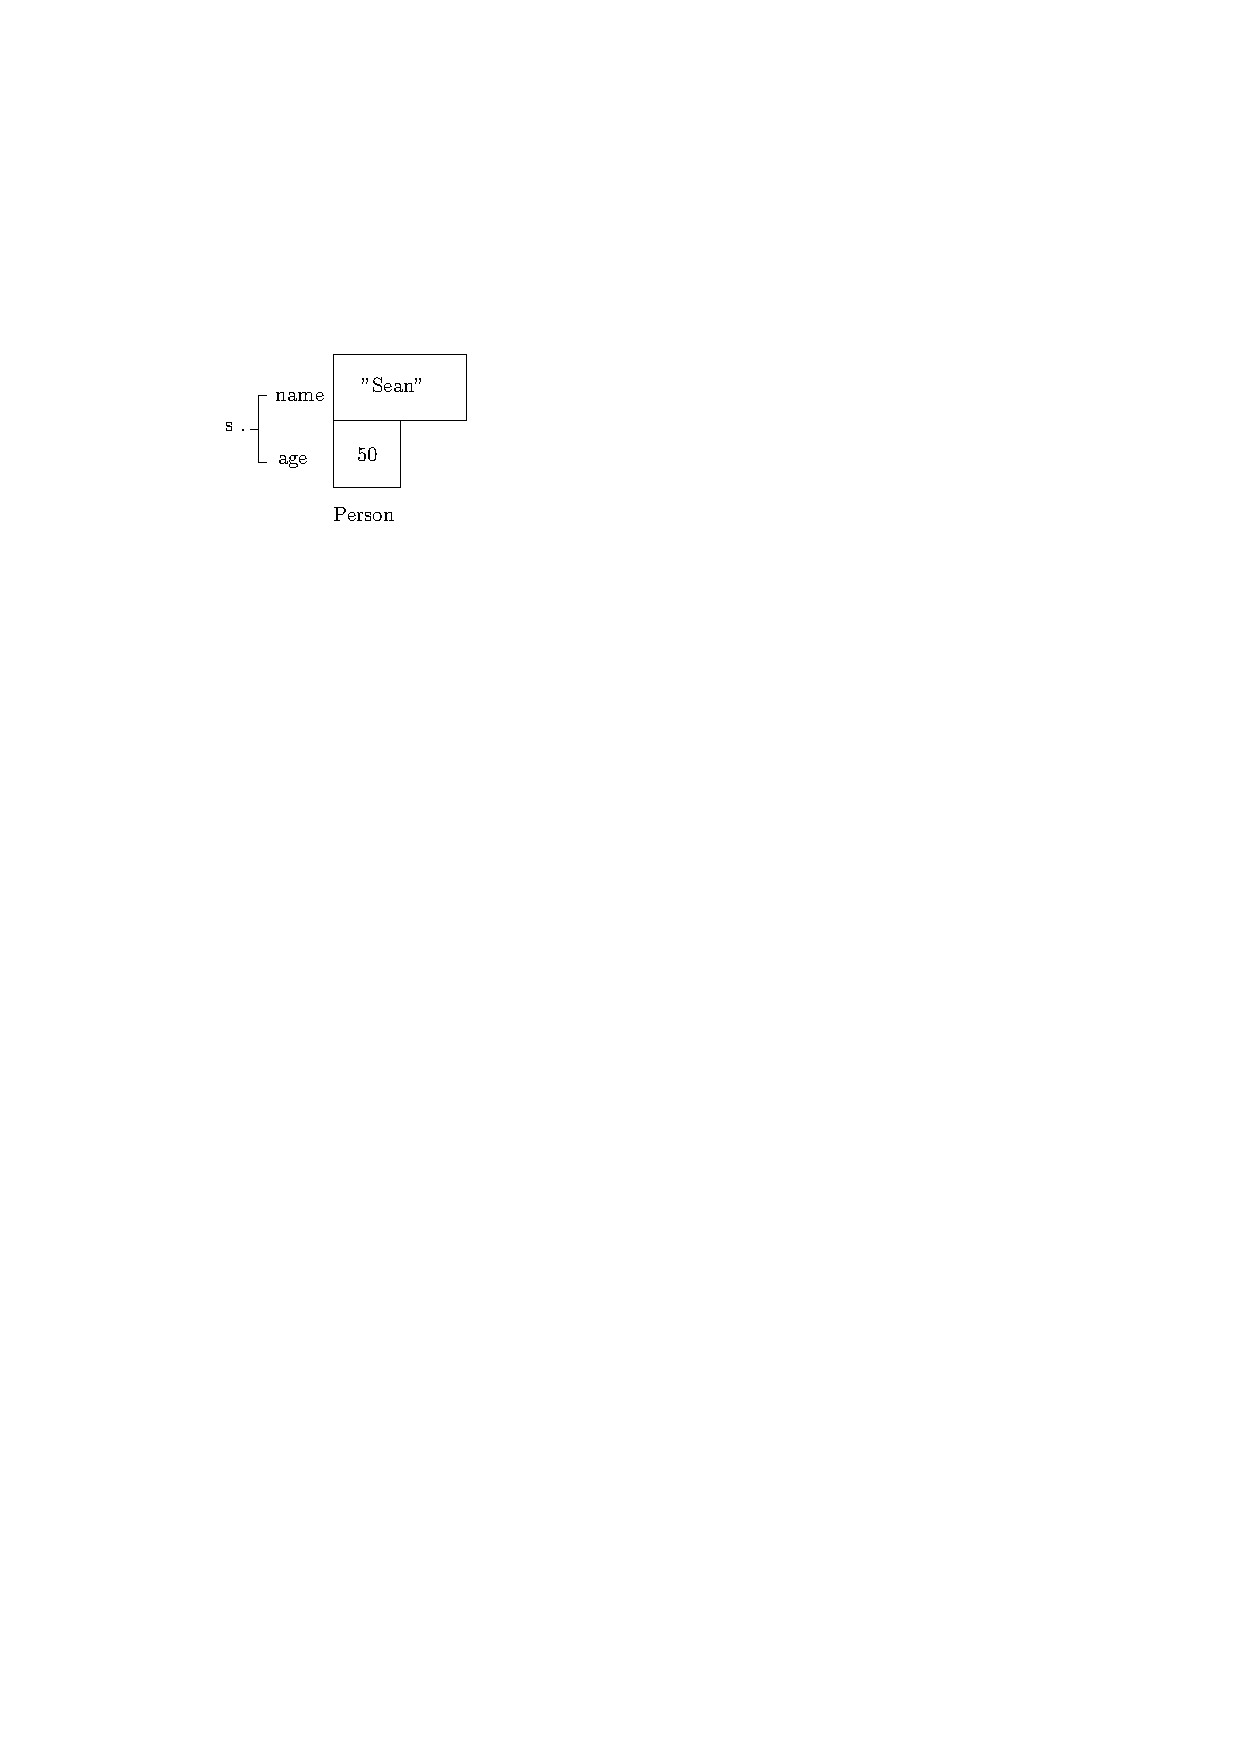
\includegraphics[width=4cm]{struct}} 
  }
  \parbox[b]{7cm}{
    \subfloat[(b)]{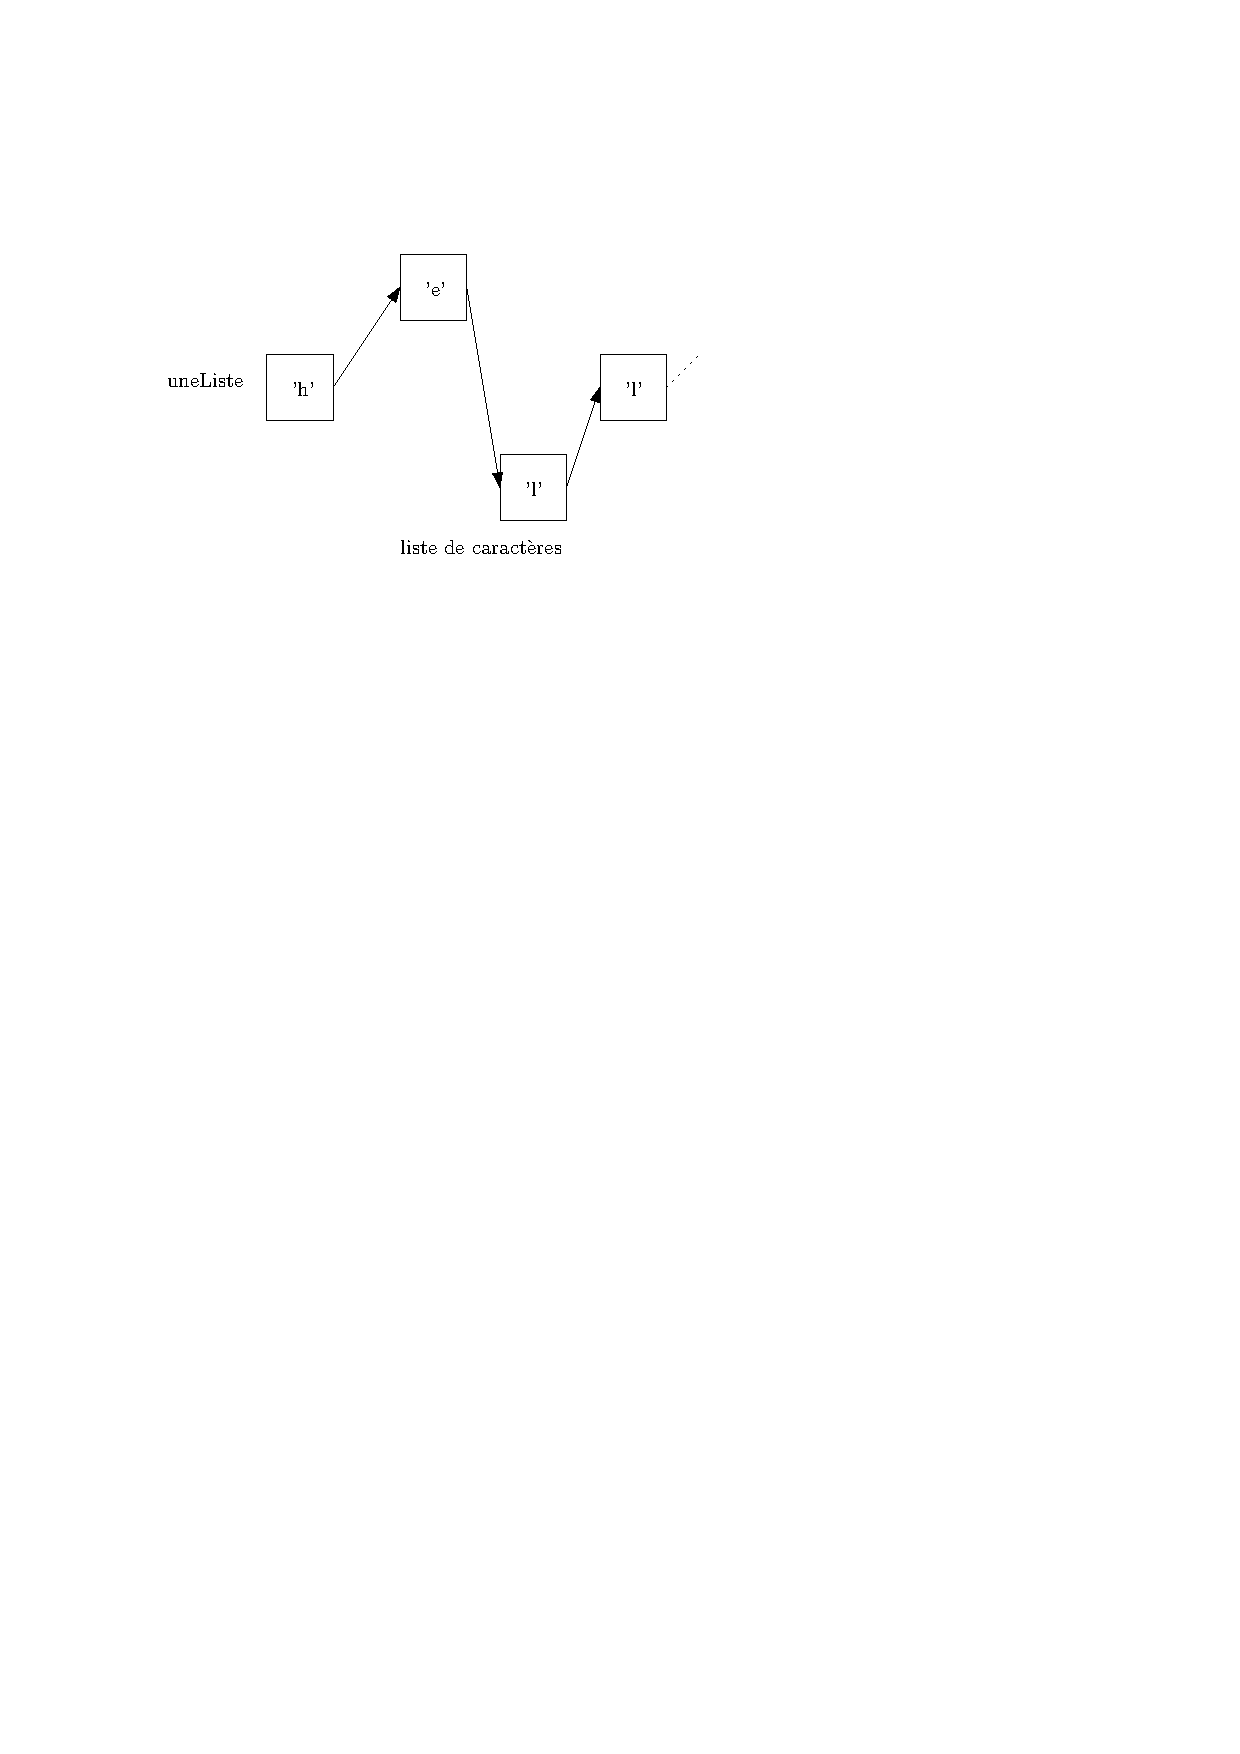
\includegraphics[width=7cm]{liste}}
  }
  \caption{Représentation schématique de valeurs structurées de type homogène en (a) et (b), non homogène en (c).}  
  \label{fig:types}
\end{figure}


\subsection{Pointeurs}

Enfin, certains langages de bas niveau, comme C ou Go, donnent la possibilité à un programme de manipuler finement la mémoire, par l'intermédiaire de \emph{pointeurs}, {\cad} de variables stockant l'adresse d'un octet en mémoire. Même si cette adresse est un entier, son utilisation particulière est facilitée par l'introduction d'un type spécifique. Le type pointeur est paramétré par un type \texttt{t} correspondant au type de la valeur localisée en mémoire à l'adresse contenue dans le pointeur. La connaissance du type \texttt{t} ne sert pas à dimensionner la boite du pointeur, qui contient une adresse codée sur 32 ou 64 bits selon l'architecture de l'ordinateur, mais sert à lire la valeur, se trouvant à l'adresse mémorisée, ou à lire d'autres valeurs adjacentes, en prenant en compte le nombre d'octets sur lesquels sont stockées ces valeurs. Un pointeur est créé à partir d'une adresse renvoyée par une fonction d'allocation mémoire ou par \emph{l'opérateur d'adresse}, souvent noté \verb!&!. L'accès à la valeur mémorisée à l'adresse contenue dans un pointeur est effectué à l'aide de \emph{l'opérateur de déréférencement}, souvent noté \verb!*!. Les variables de ce court extrait de code Go sont représentées dans la \textsc{Figure}~\ref{fig:pointeur}.  
\begin{verbatim}
x := 2          //x contient 2
p := &x         //p pointe sur x
fmt.Println(*p) //affiche 2 
\end{verbatim}

\begin{figure}[htbp]
  \centering
  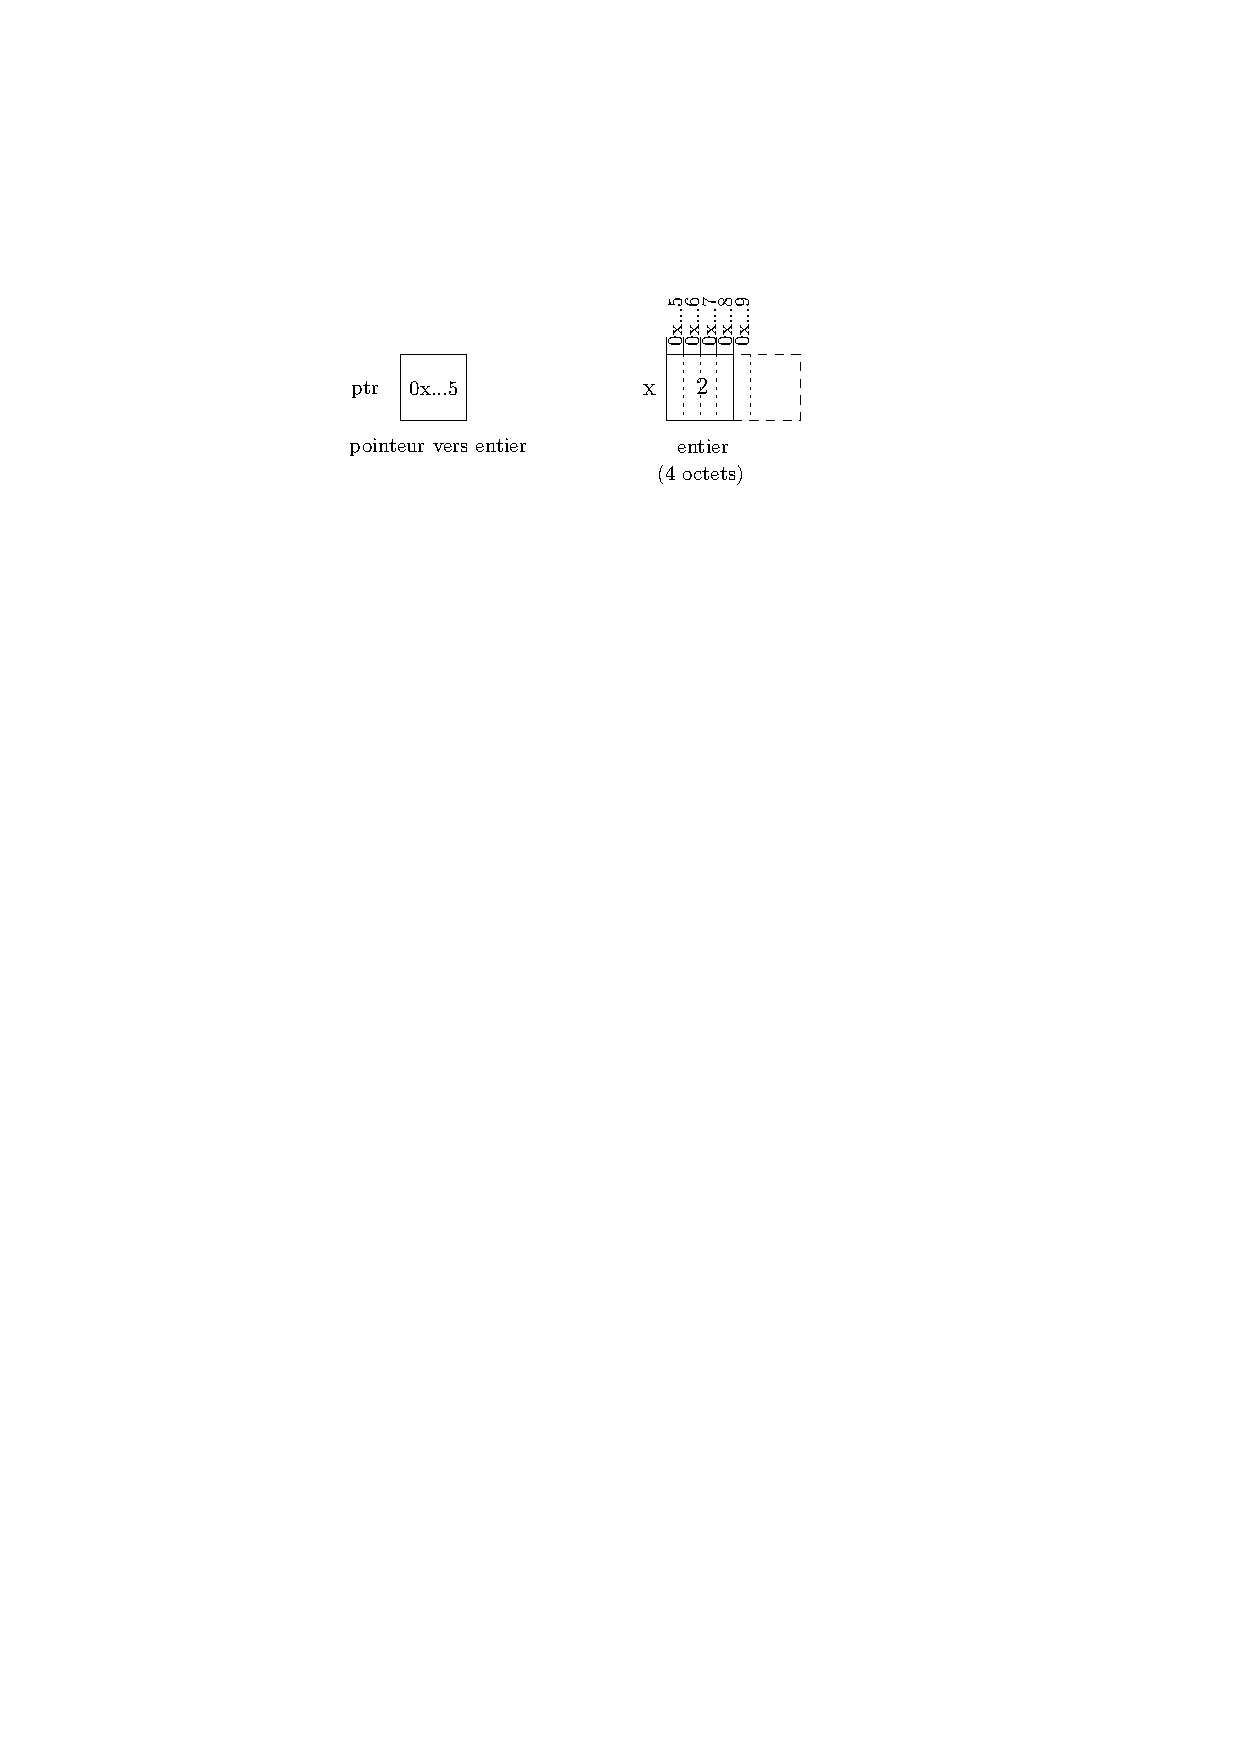
\includegraphics[width=7cm]{pointeur}
  \caption{Représentation schématique d'un pointeur.}  
  \label{fig:pointeur}
\end{figure}

Dans les langages qui les proposent, comme en C ou Go, les pointeurs sont incontournables, aussi bien pour définir et manipuler des types composés (tableau, listes, struct, arbre, graphe, etc.), qu'à d'autres niveaux, comme celui du passage de paramètres à l'appel d'une fonction (cf. section~\ref{sec:fonction}). Ce qui en fait un concept essentiel, c'est que les pointeurs sont aussi au c\oe{}ur de nombreux algorithmes et présents dans l'implémentation de nombreux autres langages qui ne permettent pourtant pas de les utiliser directement\footnote{Vous lirez certainement un message contenant \texttt{NullPointerException} en exécutant un de vos programmes Java.}.


\subsection{Typage}

Le \emph{typage} consiste à faire correspondre un type à une variable. Il peut être \emph{explicite} (le typage doit être impérativement donné dans le programme) ou \emph{implicite} (le typage n'est pas obligatoirement requis et les types possibles sont déduits automatiquement lors de la compilation ou de l'exécution). Il peut être \emph{statique} (quand le typage est établi et vérifié à la compilation) ou \emph{dynamique} (quand le typage peut être établi au cours de l'exécution). Enfin, la force du typage fait référence à la sévérité du langage quant à la combinaison de valeurs de différents types, mais cette notion est floue et il n'y a pas de définition communément admise de ce qu'est un typage fort ou faible. La \textsc{Table}~\ref{tab:typage} positionne quelques langages par rapport au typage. 
%Même si on peut dire que Haskell est fortement typé au sens où il n'y a aucune conversion implicite de type possible, alors que Javascript est faiblement typé au sens où un tout opérateur renvoie un résultat, quitte à modifier le type de l'un des opérandes.    

\begin{table}[htbp]
  \centering
\begin{tabular}{c|c|c}
  ~ & explicite & implicite \\ \hline 
  statique & C, Java & Haskell, Go \\ \hline
  dynamique & ~ & Javascript, Python
\end{tabular}
\caption{Typage de quelques langages.}
\label{tab:typage}
\end{table}


\section{Fonction}
\label{sec:fonction}

Une \emph{routine} représente un sous-programme qui, à partir d'informations données, effectue un traitement spécifique, relativement indépendant du reste du programme dans lequel il peut être réutilisé plusieurs fois. Les routines permettent de décomposer un programme en parties plus faciles à écrire, modifier, tester, réutiliser. Parmi les routines, on distingue historiquement la \emph{procédure} qui déclenche une action mais ne retourne aucune valeur, de la \emph{fonction}, qui retourne une valeur et, éventuellement, réalise une opération. On emploiera ci-dessous indifférement le mot "fonction", comme c'est le cas dans de nombreux langages.    

Une fonction possède non-seulement un sous-programme, appelé \emph{corps} ou \emph{définition}, mais aussi le plus souvent une \emph{signature}, composée d'un nom et de la liste des \emph{paramètres}, {\cad} les variables dont les valeurs devront être transmises au sous-programme \cprotect\footnote{Dans un certain nombre de langages de programmation, il actuellement possible de définir des fonctions qui n'ont pas de nom, appelées \emph{fonctions anonymes} ou \emph{fonction lambda}. C'est très pratique pour définir rapidemment de petites fonctions très spécifiques à un besoin particulier. En Haskell, par exemple, pour appliquer la fonction \texttt{f(x) = 2x + 5} à tous les éléments d'une liste, on écrit \verb!map [1,2,3,4] (\x -> 2*x + 5)!, qui est évalué en \verb![7,9,11,13]!.}. A cela, s'ajoute éventuellement un type, correspondant au type de la valeur de retour, éventuellement combiné aux types des paramètres.

Voici un exemple. Qu'elle soit définie en Go par 
\begin{verbatim}
func add(x int, y int) int {
	return x + y
}
\end{verbatim}
ou en Javascript par  
\begin{verbatim}
function add(x, y) { return x + y; }
\end{verbatim}
la fonction \texttt{add} à laquelle on fournit les valeurs \texttt{42} pour \texttt{x} et \texttt{13} pour \texttt{y} renvoie la valeur \verb!42 + 13 = 55!, ce qu'on peut noté : \verb!add(42,13)! $\leadsto$ \texttt{55}.

En Haskell, les fonctions sont généralement définies sous forme equationnelle :  
\begin{verbatim}
add x y = x + y
\end{verbatim}

Les appels sont notés sans parenthèse : \verb!add 42 13! $\leadsto$ \texttt{55}. 

\subsection{\'Evaluation stricte et paresseuse}

%expression, évaluation (paresseuse), effets vs pureté, structures de contrôle

Une \emph{expression} est un agencement de signe syntaxiquement correct (littéraux, variables, opérateurs, fonctions)
\begin{itemize}
\item qui produit éventuellement une action, qu'on appelle \emph{effet}, comme le changement de la valeur de variables en mémoire ou une opération d'entrée-sortie, 
\item et qui est \emph{évaluée} en une valeur. \footnote{
Un \emph{REPL} (pour \emph{Read-Eval-Print Loop}) est un interpréteur intéractif dans lequel l'utilisateur est invité à taper une expression (\emph{Read}). Quand celle-ci est écrite, elle est évaluée (\emph{Eval}) en un résultat, qui est ensuite affiché à l'écran (\emph{Print}), avant que l'utilisateur soit de nouveau invité à taper une expression (\emph{Loop}). C'est très pratique pour jouer avec un langage ou inspecter ce que fait certaines parties d'un programme. 
}
\end{itemize}
Le terme \emph{instruction} est généralement employé dans le cas où le résultat est ignoré et seul l'effet compte. Concrètement, \verb!2 * add(a,b+5)! est un exemple d'expression, tandis que \verb!c = add(a,b)! est un exemple d'instruction, car la valeur renvoyée par l'opérateur d'affectation est ignorée et seul l'effet, {\cad} la mise à jour de la valeur de \texttt{c}, importe.   

Il existe quelques langages, dont Haskell, dits \emph{purs}, {\cad} pour lesquels il n'y a pas d'effets (ou plutôt, ils interviennent de manière restreinte et de telle sorte qu'ils ne remettent pas fondamentalement en cause la pureté du langage). Dans ces langages, une expression donnée est toujours évaluée en une et une seule valeur, sans aucun autre effet. C'est un avantage indéniable pour comprendre, à sa simple lecture, ce que fait une partie isolée d'un programme. En revanche, les effets sont pratiques et souvent nécessaires pour atteindre une complexité algorithmique optimale, ce qui explique qu'ils sont admis et exploités par la majorité des langages de programmation.    

Cependant, la pureté offre un autre avantage. En effet, elle rend possible \emph{l'évaluation paresseuse} \cite[Lecture 6: Lazy Evaluation]{coursHaskell}, qui désigne une stratégie d'évaluation des expressions dans laquelle l'évaluation est repoussée aussi longtemps que possible. Les expressions ne sont pas évaluées tant qu'il n'est pas absolument nécessaire de le faire. Les expressions sont conservées en mémoire sous forme symbolique sans autre traitement. Par exemple, supposons que nous ayons défini en Haskell la fonction \texttt{f} telle que \verb! f x y = x + 2 !, ce qui signifie que \texttt{f} retourne la valeur de son premier paramètre augmentée de 2 (et ignore le second). L'évaluation paresseuse de l'expression \verb! f 5 (29^35792) ! n'implique pas l'évaluation de l'expression \verb! (29^35792) ! qui sera simplement stockée en mémoire sans aucun calcul et \texttt{f} sera appelée immédiatement. Puisque \texttt{f} retourne \texttt{5} sans utiliser le second argument, l'expression \verb! (29^35792) ! sera finalement supprimée sans avoir été évaluée. Au contraire, dans un langage à \emph{évaluation stricte}, évaluer \verb! f 5 (29^35792) ! exige l'évaluation de \texttt{5} (immédiate) et \verb! 29^35792 ! (ce qui nécessite un calcul coûteux) avant de passer les résultats à \texttt{f}. Dans cet exemple, le calcul coûteux s'avère finalement inutile. Mais l'avantage de l'évaluation stricte, c'est de pouvoir prédire exactement dans quel ordre les traitements se feront, ce qui est crucial quand les expressions ont des effets. C'est pourquoi l'évaluation paresseuse n'est possible qu'en l'absence d'effet.

Enfin, l'évaluation paresseuse permet de définir des \emph{structures de contrôle} comme de simples fonctions. Par exemple, la structure de contrôle \texttt{if} évalue ou exécute, parmi deux alternatives, seulement l'une d'elles, selon la valeur d'une condition. En Haskell, l'évaluation paresseuse permet de définir cette structure de contrôle à l'aide d'une simple fonction. La fonction \texttt{if} est définie de telle sorte que pour évaluer \verb! if condition a b !, seulement l'expression \texttt{a} est évaluée si \texttt{condition} est évaluée à vrai, tandis que l'expression \texttt{b} n'est pas utilisée, et inversement si \texttt{condition} est évaluée à faux. Au contraire, dans les langages à évaluation stricte, tous les arguments d'une telle fonction seraient évalués, ce qui serait absurde. C'est pourquoi, il existe dans ces langages des constructions spécifiques pour les structures de contrôle qui fonctionnent et sont nommées à peu près toujours de la même manière :
\begin{description}
\item[branchement] \verb! if / then / else / elif !, \verb! switch / case / break !, 
\item[boucle] \verb! for / break / continue !, \verb! while !, \verb! do while !.
\end{description}

\subsection{\'Evaluation stricte et modalité de passage de paramètre}

Reprenons l'exemple de la fonction \texttt{add} définie précédemment. L'évaluation de \verb!add(a,b+5)! nécessite deux actions. D'une part, mettre en correspondance les \emph{paramètres effectifs} (ou encore \emph{arguments}) \texttt{a} et \texttt{b+5} aux \emph{paramètres formels} de la définition (ou plus simplement paramètre), \texttt{x} et \texttt{y}. Le i-ème argument de la liste d'appel est toujours associé au i-ème paramètre de la signature. D'autre part, pour chaque couple argument et paramètre, s'arranger pour que le paramètre représente une variable contenant le résultat de l'évaluation de l'argument. Il existe différentes possibilités, mais on n'en côtoie couramment que deux, la première est largement majoritaire : il s'agit du passage de paramètre par copie (\emph{call-by-value}) et du passage de paramètre par référence (\emph{call-by-reference}).

Le passage de paramètre par copie consiste, pour chaque couple argument et paramètre, à créer une variable contenant une copie de la valeur de l'argument et à lui donner le nom du paramètre (\textsc{Figure}~\ref{fig:passage} (a)). Le passage de paramètre par référence consiste tout simplement à enregistrer le nom du paramètre comme désignant la variable contenant la valeur de l'argument (\textsc{Figure}~\ref{fig:passage} (b)). La différence est déterminante dans la façon de programmer puisque dans le second cas, une instruction du corps de la fonction peut modifier la valeur d'un argument (par exemple \texttt{a}, via \texttt{x}), alors que c'est impossible dans le premier cas du fait de la copie. 

\captionsetup[subfigure]{labelformat=parens}
\begin{figure}[htbp]
  \centering
  \subfloat[]{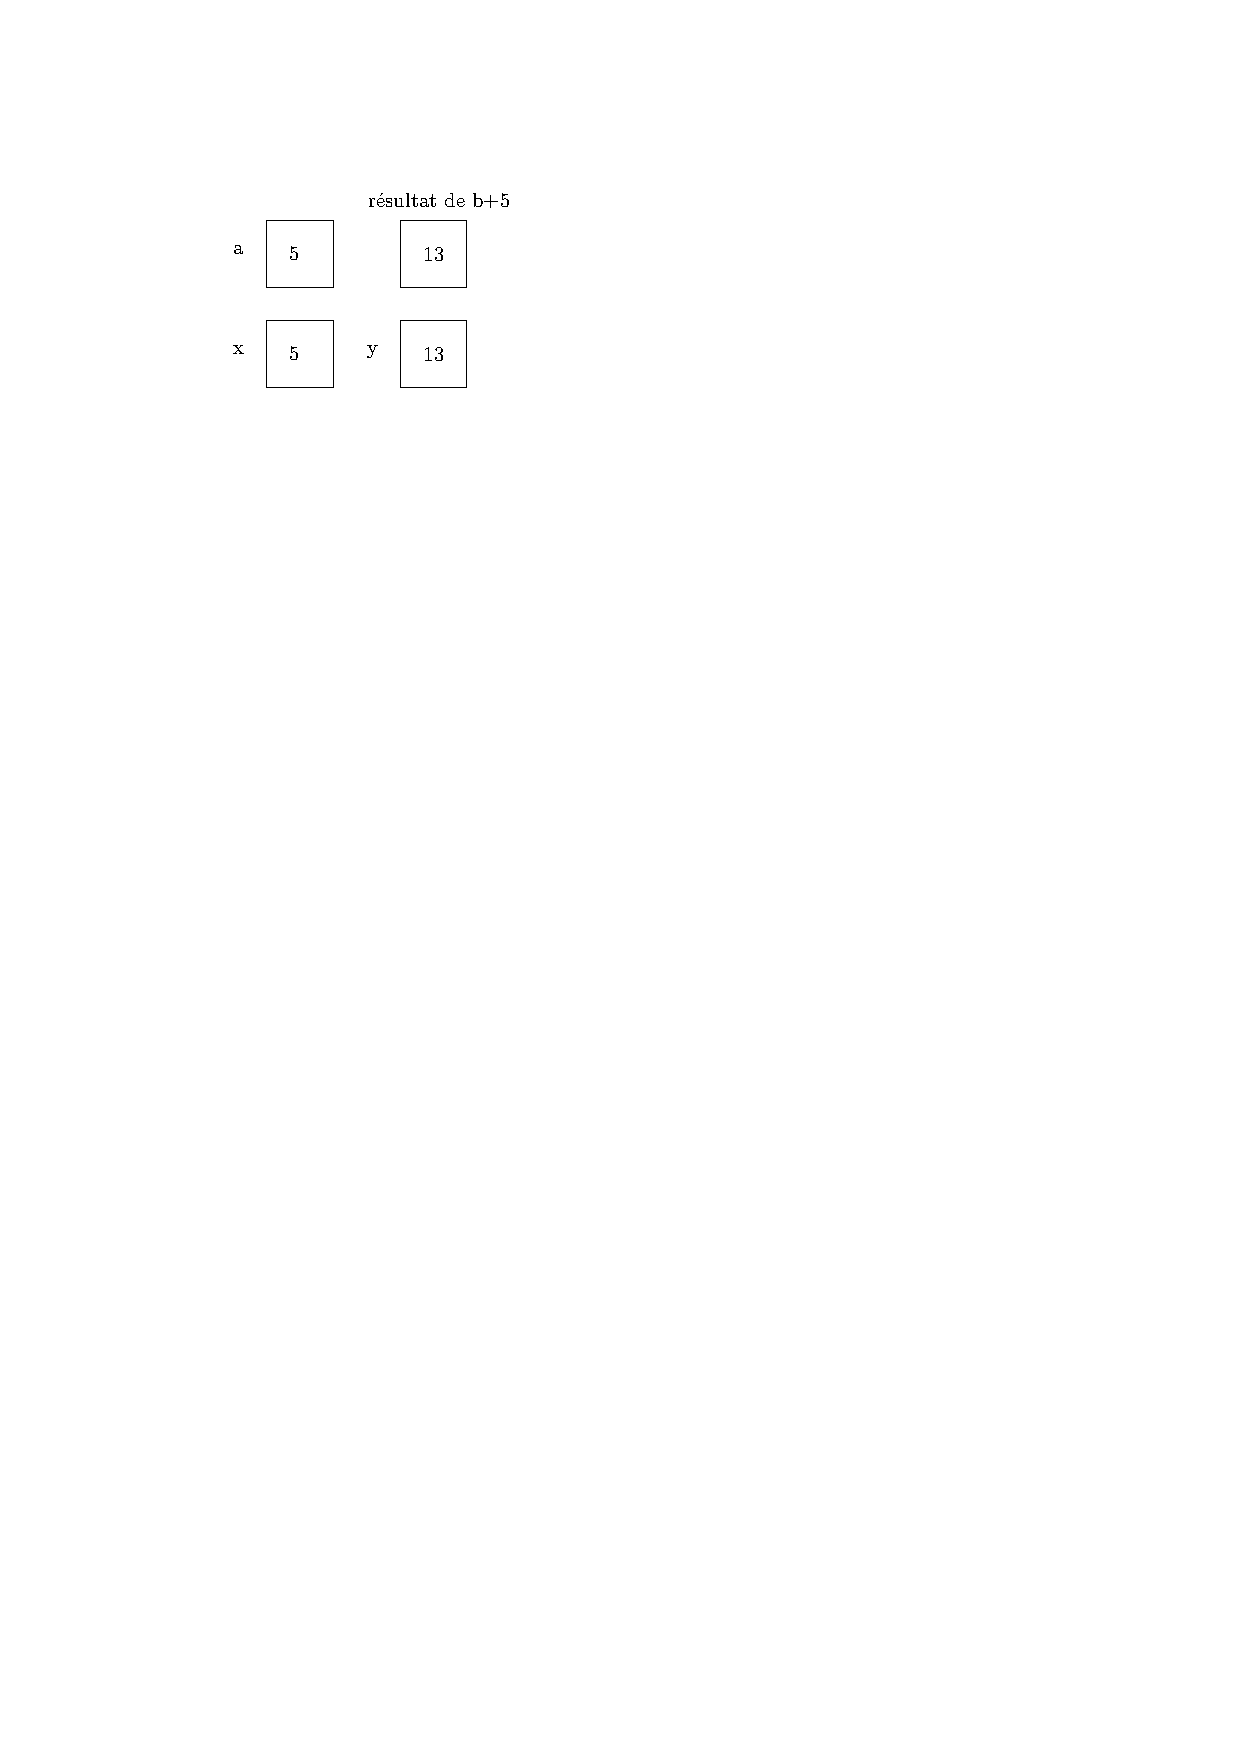
\includegraphics[width=4cm]{callByValue}} \hspace{1cm}
  \subfloat[]{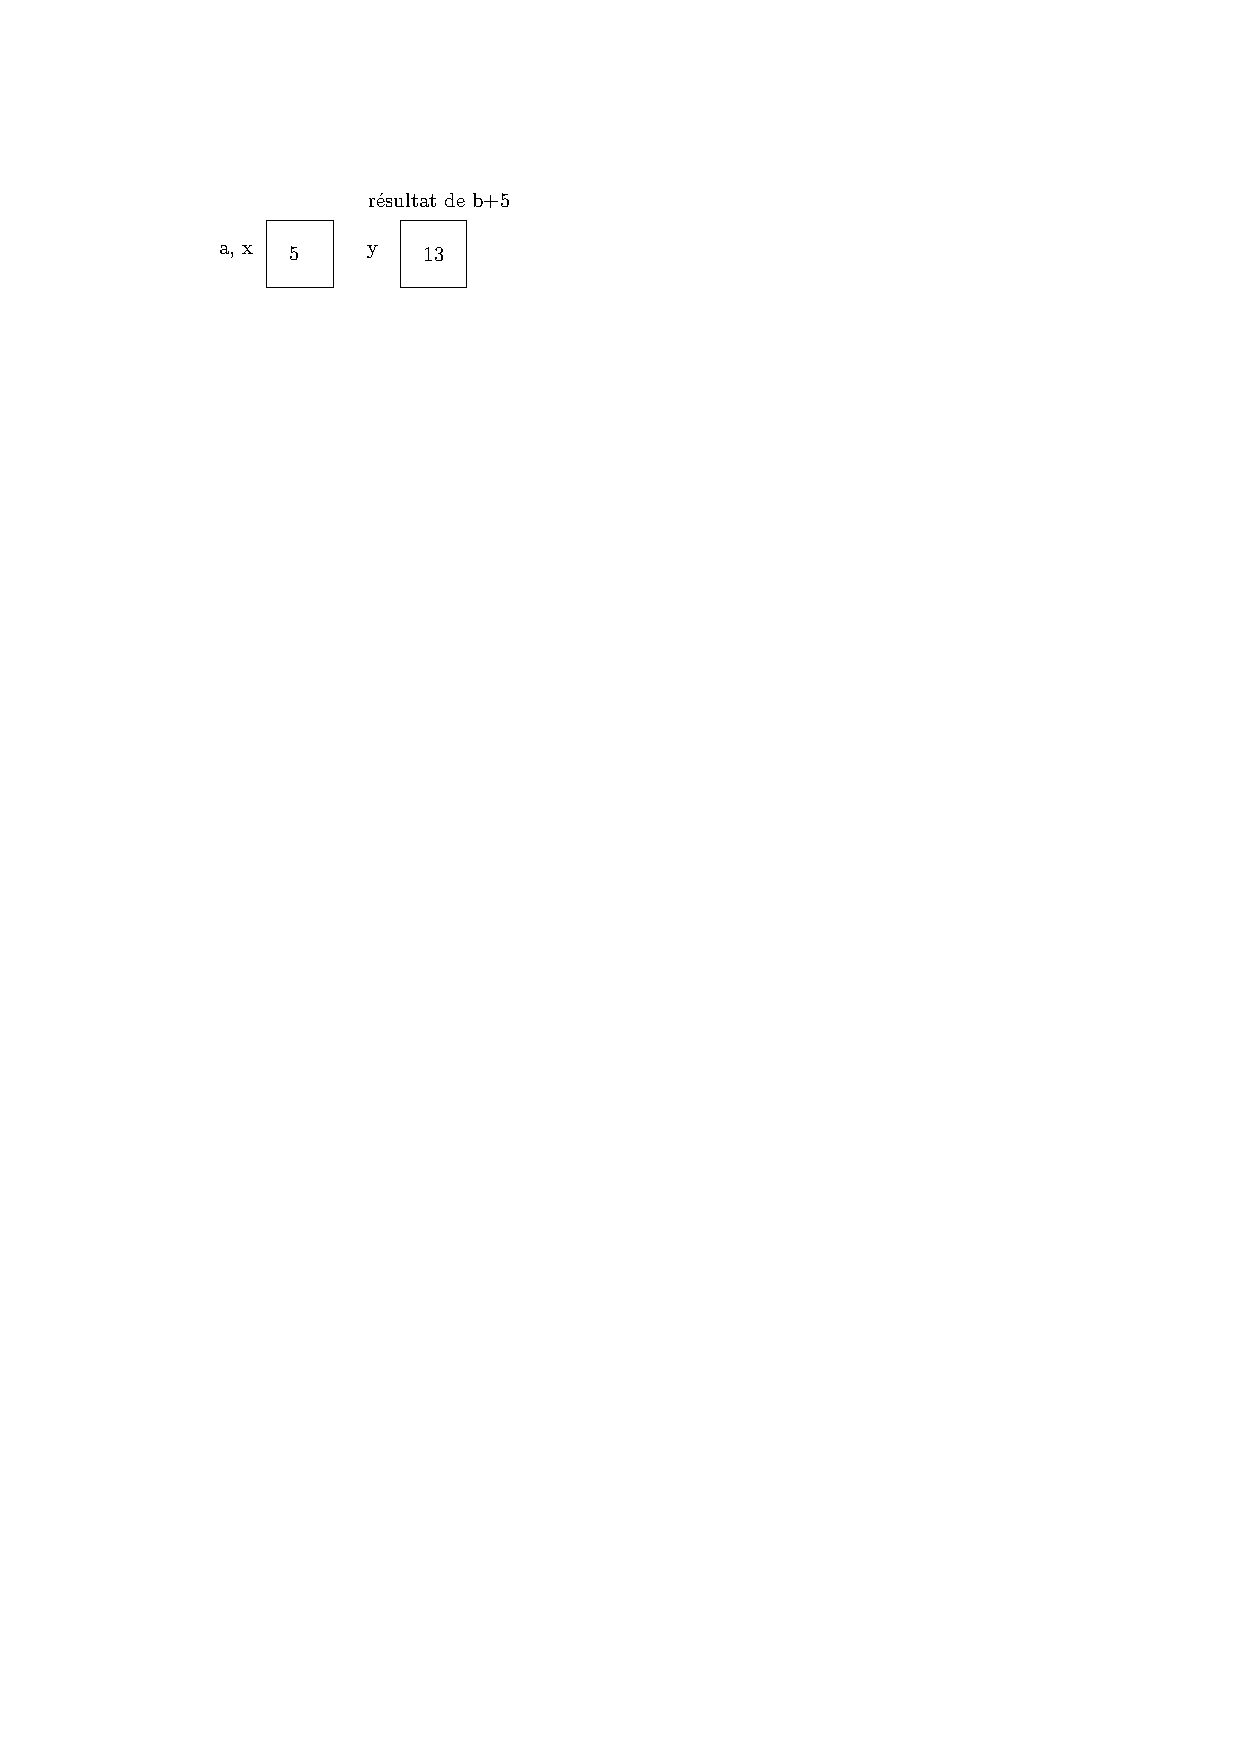
\includegraphics[width=4cm]{callByRef}} 
  \caption{Passage de paramètre par copie en (a) et par référence en (b).}  
  \label{fig:passage}
\end{figure}

Ce qui est trompeur, c'est que les arguments peuvent être des pointeurs ou assimilés. L'utilisation de pointeurs dans le cas d'un passage de paramètre par copie donne l'illusion d'un passage de paramètre par référence, car des instructions du corps de la fonction pourront modifiées des valeurs pointées. Un test imparable consiste à vérifier s'il est possible de permuter les valeurs des arguments (un exemple est détaillée en annexe~\ref{a:passage}). 

\subsection{\'Evaluation partielle}

La programmation fonctionnelle propose une série de concepts très puissants qui découlent pourtant de cette simple posture : la fonction est considérée comme une valeur comme une autre. En conséquence, une fonction peut avoir des fonctions comme paramètres ou retourner une fonction. Dans ce cas, elle est qualifiée \emph{d'ordre supérieur}. Il s'ensuit qu'une fonction à plusieurs paramètres peut de manière equivalente être considérée comme une fonction à un paramètre, qui retourne une fonction paramétrée uniquement par les paramètres suivants. C'est ce qu'on appelle la \emph{curryfication}, en référence au logicien Haskell Curry. Une conséquence directe est qu'il est possible d'évaluer \emph{partiellement} une fonction à plusieurs paramètres en ne donnant que le premier argument. Dans ce cas, on obtient une fonction avec un paramètre de moins, comme si, dans le corps de la fonction de départ, le premier paramètre avait été remplacé par la valeur fournie. La capture de valeurs accompagnant une fonction, comme c'est le cas lors d'une évaluation partielle, est appelée \emph{fermeture} (ou \emph{closure} en anglais). 

En Haskell, nous pouvons par exemple écrire
\begin{verbatim}
add x y = x + y
add42 = add 42 -- évaluation partielle 
\end{verbatim}
\'Evidemment \verb!add42 5! est évalué en \texttt{47}. En revanche \verb!add 42! est évaluée en une fonction qui prend en entrée une valeur pour son paramètre \texttt{y} et retourne la somme de cette valeur et de celle mémorisée pour \texttt{x}, {\cad} \texttt{42}. Nous avons donc l'égalité suivante : \verb!add42 = \y -> 42 + y!. 


\subsection{Fonction vs méthode}
\label{sec:fonction-methode}

Classiquement en programmation orientée objet, une \emph{classe} décrit à la fois la structure d'une variable composée, ainsi que les opérations possibles sur cette variable. La structure est définie par un ensemble de \emph{champs}, comme dans un type composé (section~\ref{sec:types-composes}). Les opérations sont définies par un ensemble de fonctions, appelées \emph{méthodes} dans ce contexte. Une telle variable est appelée \emph{objet}. Son \emph{état} est donné par les valeurs de ses champs, tandis que son \emph{comportement} est codé par les méthodes.   

L'intérêt de cette approche est principalement de regrouper toutes les opérations qui s'appliquent à un même type de valeur. Prenons l'exemple de la modélisation d'une file. Plusieurs opérations s'appliquent à une file, notamment ajouter un élément en dernière position, au bout de la file (\texttt{enfiler}), supprimer le premier élément de la file et le retourner (\texttt{sortir}). Au lieu d'écrire deux fonctions indépendantes requérant chacune une variable de type \texttt{File} comme paramètre, la programmation orientée objet propose d'attacher ces fonctions au type \texttt{File} en sachant que leur appel aura lieu dans un contexte contenant une variable de type \texttt{File}. Concrètement, voici une comparaison de ces deux stratégies en Python.

~

\begin{minipage}[c]{0.45\textwidth}
\begin{verbatim}
#fonctions indépendantes
class File:
  ...

def enfiler(uneFile, unElt):
  ...
def sortir(uneFile):
  ...
\end{verbatim}
\begin{verbatim}
f = File()
...
enfiler(f, 5)
premier = sortir(f)
\end{verbatim}
\end{minipage}
%
\hfill\vline\hfill
%
\begin{minipage}[c]{0.45\textwidth}
\begin{verbatim}
#méthodes de File
class File(object):
  def enfiler(self, unElt):
    ...
  def sortir(self):
    ...
\end{verbatim}

\vspace{0.4cm}

\begin{verbatim}
f = File()
...
f.enfiler(5)
premier = f.sortir()
\end{verbatim}
\end{minipage}

~

Bien que fonction et méthode soient presques synonymes, il y a cependant deux différences entre ces deux concepts. La première différence, c'est que la méthode s'applique toujours sur au moins une variable, qui est en général un objet. La seconde différence, c'est que l'action déclenchée par l'appel à une méthode depuis un objet dépend de la catégorie de l'objet en question. Ce mécanisme est détaillé dans la section suivante. 

\section{Polymorphisme}

- polymorphisme (interface/héritage, classe de type)

\section{Organisation du code source et conflits de nom}

A FAIRE

\section{Erreurs et exceptions}

A FAIRE

\section{Parallélisme et concurrence}

A FAIRE

\section{Paradigmes de programmation}

- impératif, (CRO)
- fonctionnel, 
- objet, 
- concurrent, (PPC)

%annexes
\appendix
\section{Enregistrements}
\label{a:enregistrement}

Voici différents morceaux de code correspondant à la \textsc{Figure}~\ref{fig:types}(c).

\subsection{Haskell}

En Haskell, il est tout aussi possible de nommer les champs
\begin{verbatim}
data Person = Person {
    name :: String, 
    age :: Int
}
s = Person {nom="Sean", age=50}
\end{verbatim}
ou non...
\begin{verbatim}
data Person = Person String Int
s = Person "Sean" 50
\end{verbatim}
et même d'exploiter le type tuple déjà défini en lui donnant un synonyme.
\begin{verbatim}
type Person = (String, Int)
s = ("Sean", 50)
\end{verbatim}

\subsection{Go}

\begin{verbatim}
type Person struct {
    name string
    age  int
}    
s := person{name: "Sean", age: 50}
\end{verbatim}

\subsection{Java}

En java, il est nécessaire d'écrire soi-même la fonction qui crée en mémoire une variable contenant les données requises. Il existe un constructeur par défaut, mais celui-ci ne fait rien de plus que l'initialisation des champs à des valeurs par défaut (zéro binaire). Cette fonction particulière est appelée \emph{constructeur} et la variable \emph{objet} ou \emph{instance}. 
\begin{verbatim}
class Person {
  String name; 
  int age; 
  Person(String givenName, int givenAge) {
    name = givenName;
    age = givenAge;
  }
}
\end{verbatim}

Toute construction est effectuée à l'aide de l'opérateur \texttt{new}.  
\begin{verbatim}
s = new Person("Sean", 50);  
\end{verbatim}

L'appel à cet opérateur implique la création de l'objet en mémoire, puis le renvoi d'une valeur, servant d'intermédiaire pour accéder à l'objet (à la manière d'un pointeur).

\subsection{Javascript}

En Javascript, il est possible d'appliquer l'opérateur \texttt{new} sur une fonction faisant office de constructeur.
\begin{verbatim}
function Person (givenName, givenAge) {
    this.name = givenName; 
    this.age = givenAge; 
}
let s = new Person("Sean", 50)
\end{verbatim}
L'appel à cet opérateur implique la création d'un nouvel objet en mémoire et sa mise en correspondance avec un autre objet, son \emph{prototype}, qui est par défaut \verb!{}!. Les prototypes sont chainés jusqu'à la valeur spéciale \texttt{null}. Au nouvel objet, désigné par \texttt{this}, sont ajoutés dynamiquement de nouveaux champs. La valeur renvoyée par \texttt{new}, n'est pas l'objet lui-même, mais un identifiant pour accéder à celui-ci.
%Attention, malgré la similarité syntaxique avec Java, Javascript est très différent dans son fonctionnement.

%cf. 
%https://blog.xebia.fr/2013/06/10/javascript-retour-aux-bases-constructeur-prototype-et-heritage/
%https://developer.mozilla.org/fr/docs/Web/JavaScript/H%C3%A9ritage_et_cha%C3%AEne_de_prototypes


\section{Passage de paramètre et objets}
\label{a:passage}

Prenons l'exemple du langage Java pour voir ce que donne le passage de paramètre par copie dans le cas de variables assimilables à des pointeurs. 

La classe \texttt{A} ci-dessous est dotée d'un champs entier, nommé \texttt{myA} :
\begin{verbatim}
class A {
  public int content;
  public A(int a) {
    content = a;
  }
  @Override
  public String toString() {
    return super.toString() + " contient " + content; 
  }
}
\end{verbatim}

Dans le code ci-dessous, nous créons deux objets de type \texttt{A} contenant respectivement \texttt{1} et \texttt{2}. Les deux variables \texttt{unA1} et \texttt{unA2}, comme des pointeurs, sont des intermédiaires procurant un accès aux objets créés, mais non les objets eux-mêmes. Pour l'observer, nous appelons la méthode \texttt{foo}, qui fait deux actions : elle permute les valeurs de ses deux paramètres, puis remplace le contenu du premier paramètre (donc du second à cause de l'échange) par \texttt{5}. 

\begin{verbatim}
public class CallByValueWithObj {
  public static void foo(A a1, A a2) {
    A tmp = a1;
    a1 = a2;
    a2 = tmp;
    a1.content = 5;
  }
  public static void main(String args[]) {
    A unA1 = new A(1);
    A unA2 = new A(2);
    System.out.println(unA1 + " " + unA2);
    foo(unA1, unA2);	
    System.out.println(unA1 + " " + unA2);	
  }
}
\end{verbatim}

\`A l'exécution, voici ce qu'on peut lire :

\begin{verbatim}
A@15db9742 contient 1 A@6d06d69c contient 2
A@15db9742 contient 1 A@6d06d69c contient 5
\end{verbatim}

Les deux objets n'ont pas été échangés, ce qui signifie qu'il s'agit bien d'un passage par copie. Cependant, il est à tout à fait possible de modifier le contenu des objets car ce sont les intermédiaires vers les objets créés et non les objets eux-mêmes qui sont copiés. 

\bibliographystyle{plain}
\bibliography{refs}

\end{document}


